% $Id: State_implnotes.tex,v 1.6 2006/02/01 18:56:28 cdeluca Exp $
%
% Earth System Modeling Framework
% Copyright 2002-2003, University Corporation for Atmospheric Research, 
% Massachusetts Institute of Technology, Geophysical Fluid Dynamics 
% Laboratory, University of Michigan, National Centers for Environmental 
% Prediction, Los Alamos National Laboratory, Argonne National Laboratory, 
% NASA Goddard Space Flight Center.
% Licensed under the GPL.

%\subsection{Design and Implementation Notes}

\begin{enumerate}

\item
States contain the name of the associated Component, a flag for Import
or Export, and a list of data objects, which can be a combination of
Bundles, Fields, and/or Arrays.  The objects must be named and have
the proper attributes so they can be identified by the receiver of
the data.  For example, units and other detailed information
may need to be associated with the data as an Attribute.  

\item
Data contained in States must be created in unison on each
PET of the current VM.  This allows the creation process to avoid
doing communications since each PET can compute any information
it needs to know about any remote PET (for example, the grid
distribute method can compute the decomposition of the grid on
not only the local PET but also the remote PETs since it knows
each PET is making the identical call).  For all PETs to have a
consistent view of the data this means objects must be given
unique names when created, or all objects must be created in
the same order on all PETs so ESMF can generate consistent
default names for the objects.

When running components on subsets of the original VM all the
PETs can create consistent objects but then when they are put
into a State and passed to a component with a different VM and
a different set of PETs, a communication call (reconcile) must be 
made to communicate the missing information to the PETs which were 
not involved in the original object creation.  The reconcile call
broadcasts object lists; those PETs which are missing any objects
in the total list can receive enough information to
reconstruct a proxy object which contains all necessary information
about that object, with no local data, on that PET.  These proxy
objects can be queried by ESMF routines to determine the amount
of data and what PETs contain data which is destined to be moved
to the local PET (for receiving data) and conversely, can determine
which other PETs are going to receive data and how much (for
sending data).

For example, the FieldExcl system test creates 2 gridded components
on separate subsets of PETs.  They use the option of mapping
particular, non-monotonic PETs to DEs.  The following figures 
illustrate how the DEs are mapped in each of the gridded components
in that test:

\begin{center}
\begin{figure}
\scalebox{0.9}{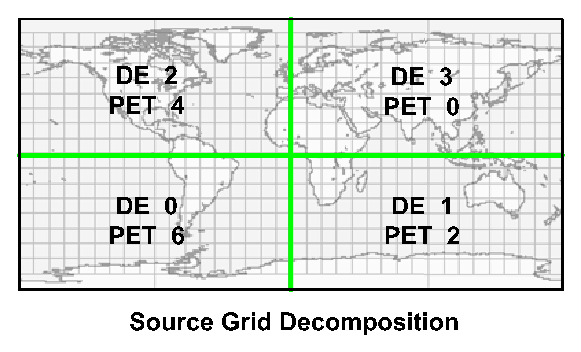
\includegraphics{Excl_src_grid}}
\caption{The mapping of PETs (processors) to DEs (data)
in the source grid created by {\tt user\_model1.F90}
in the FieldExcl system test.}
\label{fig:excl_source}
\end{figure}
\end{center}

\begin{center}
\begin{figure}
\scalebox{0.9}{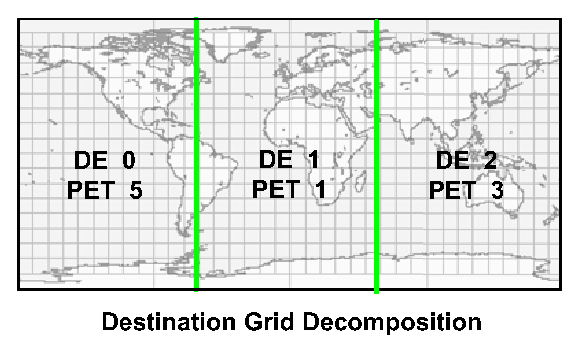
\includegraphics{Excl_dst_grid}}
\caption{The mapping of PETs (processors) to DEs (data)
in the destination grid created by {\tt user\_model2.F90}
in the FieldExcl system test.}
\label{fig:excl_destination}
\end{figure}
\end{center}

In the coupler code, all PETs must make the reconcile call before
accessing data in the State.  On PETs which already contain data,
the objects are unchanged.  On PETs which were not involved during
the creation of the Bundles or Fields, the reconcile call adds an
object to the State which contains all the same metadata associated
with the object, but creates a slightly different Grid object,
called a Proxy Grid. These PETs contain no local data, so the
Array object is empty, and the DELayout for the Grid is like this:

\begin{center}
\begin{figure}
\scalebox{0.9}{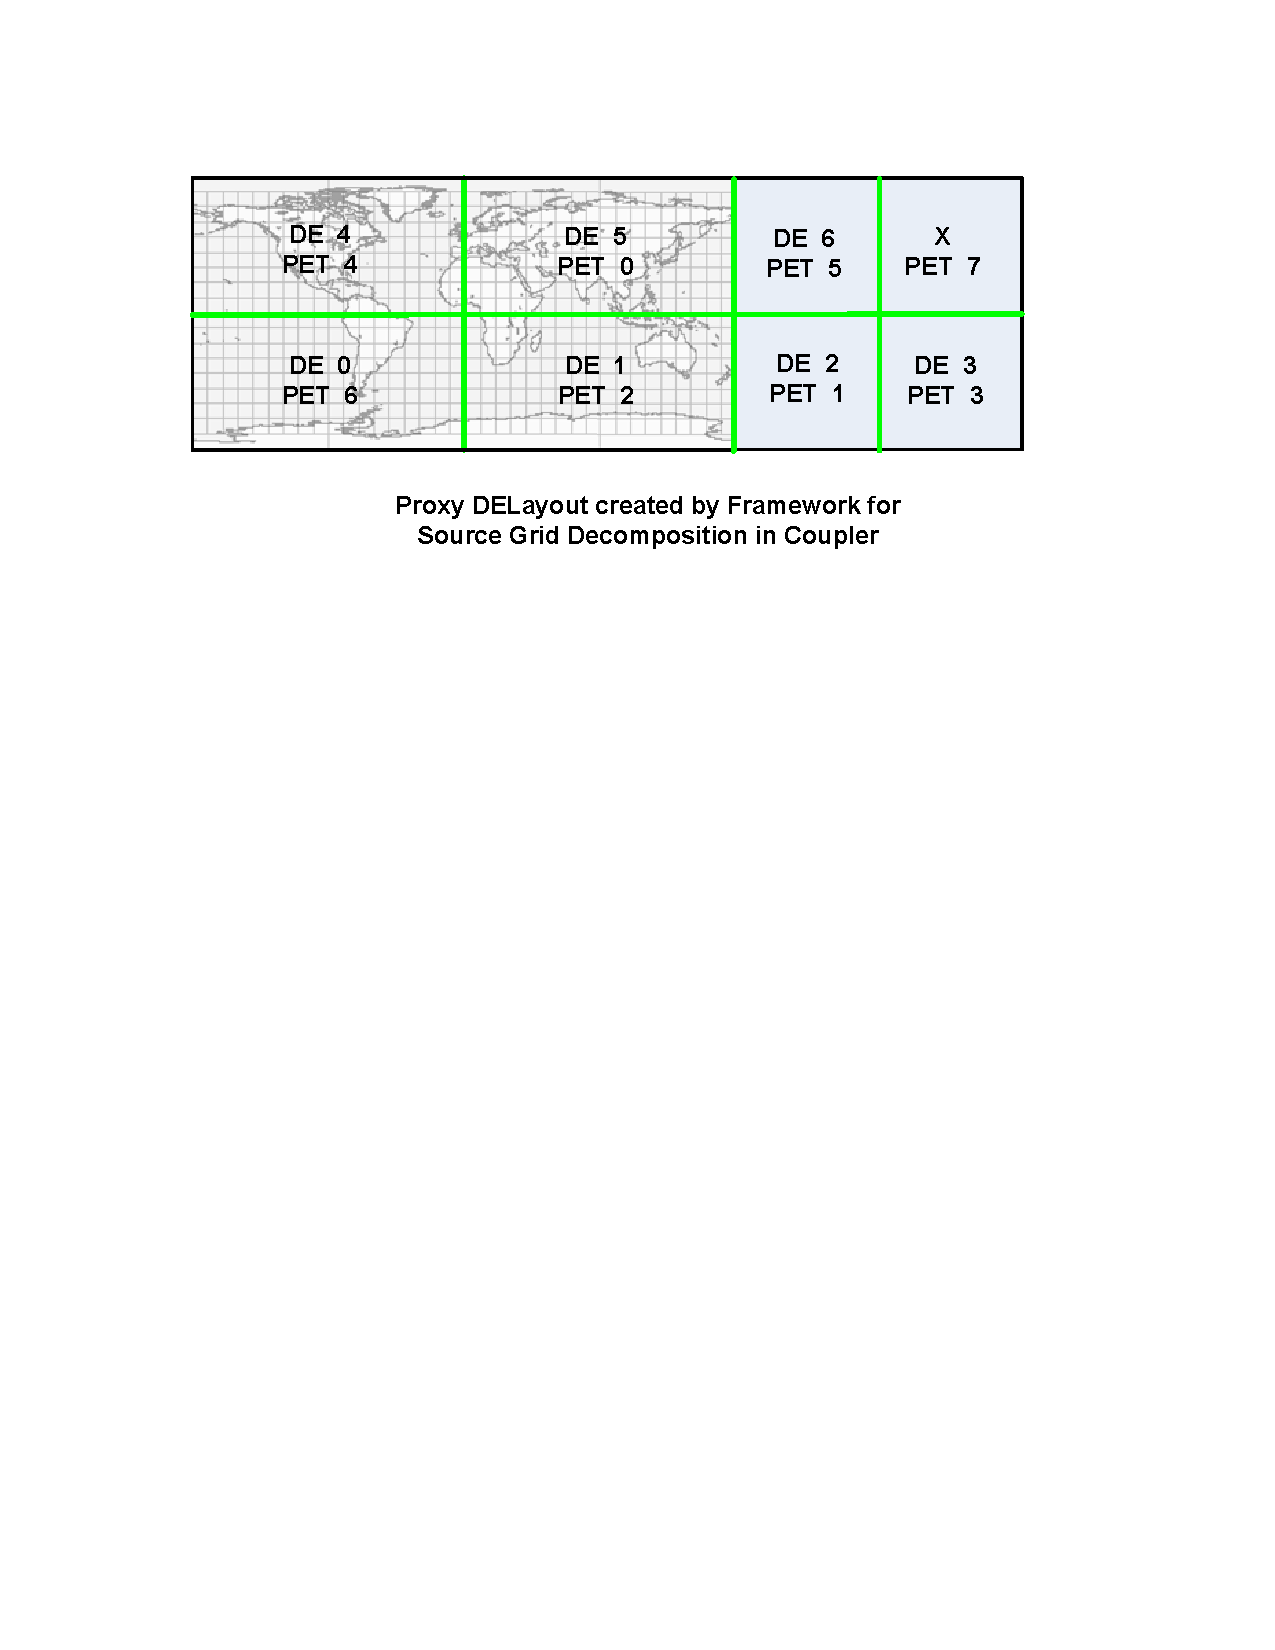
\includegraphics{Excl_src_grid_cpl}}
\caption{The mapping of PETs (processors) to DEs (data)
in the source grid after the reconcile call in {\tt user\_coupler.F90}
in the FieldExcl system test.}
\label{fig:excl_source}
\end{figure}
\end{center}

\begin{center}
\begin{figure}
\scalebox{0.9}{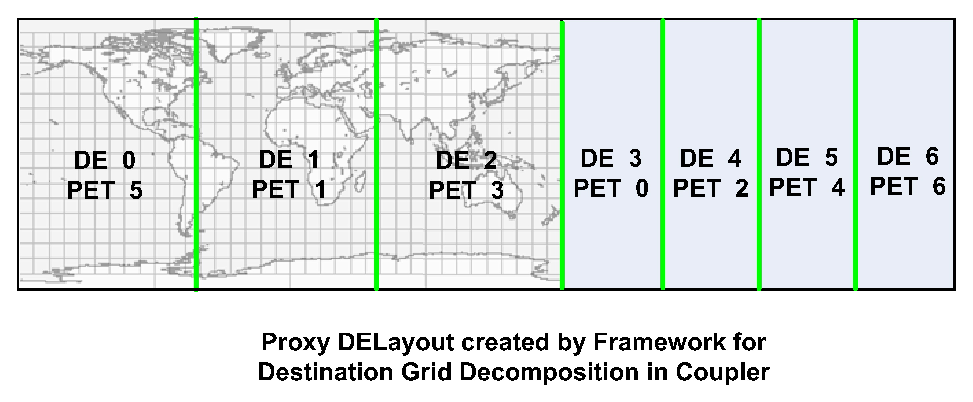
\includegraphics{Excl_dst_grid_cpl}}
\caption{The mapping of PETs (processors) to DEs (data)
in the destination grid after the reconcile call in {\tt user\_coupler.F90}
in the FieldExcl system test.}
\label{fig:excl_destination}
\end{figure}
\end{center}

\end{enumerate}
